%% IMPORTANT: Once working, run latex 3 times to get listoffigures to work

%% Be sure to check spelling!

%% Put **your** name and the proper due date in place

%% Note put your own file names in the appendix
%% Copy the relevant code as many times as needed for all files

%% Note that the \epsfig command is currently commented out

\documentclass{article}
\usepackage{amsmath}    % load AMS-Math package
\usepackage{epsfig}     % allows PostScript files
\usepackage{listings}   % allows lstlisting environment
\usepackage{moreverb}   % allows listinginput environment
\usepackage{vmargin}    % allows better margins
\setpapersize{USletter} % sets the paper size
\usepackage[table]{xcolor}
\setmarginsrb{1in}{0.5in}{1in}{0.2in}{12pt}{11mm}{0pt}{11mm} %sets margins 
\begin{document}
\begin{center}
\rule{6.5in}{0.5mm}\\~\\
{\bf \large EGR 103L - Fall 2016}\\~\\
{\huge \bf Laboratory 5 - Graphical Methods}\\~\\
CEMAL YAGCIOGLU (cy111)\\
Lab Section 5D, Wednesday 11.45AM - 2.35PM\\
16 OCTOBER, 2016\\~\\
{\small I understand and have adhered to all the tenets of the Duke
  Community Standard in completing every part of this assignment.  I
  understand that a violation of any part of the Standard on any part
  of this assignment can result in failure of this assignment, failure
  of this course, and/or suspension from Duke University.} 
\rule{6.5in}{0.5mm}\\
\end{center}
\tableofcontents
\listoffigures
\pagebreak

\section{Palm Problem 5.3(a)}
Roots are -0.479,1.135,3.832.

\section{Palm Problems 5.21 and 6.7}
Bar and stairs graphs have  continous x domains that might suggest that the potential value stays same for a short peroiod of time and instantly drops. However, data does not suggest an instant change of potential. Thus, it rather makes more sense to have the stem graph with more accurate point data. 

\section{Chapra Problem 3.9}
Increasing depth and width increases the velocity of water. Depth seems to have slightly more weight on velocity value. As depth and width increases, change in velocity(slope of the tangent plane) decreases.  

\section{Palm Problem 5.33}
At point x=y=0, Temperature is 1.4653 Kelvin.

\section{Palm Problem 5.36}
Surface graph is drawn and added to the document.

\section{Palm Problem 4.28}
Coordinate for the lowest-cost distribution center is (8,2) and the cost for that location is 4.1180e+02.
\begin{center}
\begin{tabular}{cccc}
\hline
\textbf{Customer} & \textbf{xlocation(mi)} & \textbf{ylocation(mi)} & \textbf{Volume(tons/week)}\\
\hline
   1 &    29 &   6 &  8 \\
   2  &  -20 &  -12 &  6 \\
   3   &   9 &  1 &  4 \\
   4   &   1 &  29 &  2 \\
   5   &  -3 &  21 &  5 \\
   6   &  11 &  3 &  8 \\
   7  &  -15 &  -5 &  5 \\
   8  &    5 &  -9 &  2 \\
   9  &  -26 &  13 &  3 \\
  10   &  14 & 19 &  1 \\
\hline
\end{tabular}
\end{center} 
\section{Codes and Output}
% Put the name of your file in the subsection name 
% and the listinginput input
% Be sure to include the community standard in codes!
% Add \pagebreaks if they make sense
% Make as many copies as you need

\subsection{ThreeRoots.m}
\listinginput[1]{1}{ThreeRoots.m}

\subsection{VoltageCalc.m}
\listinginput[1]{1}{VoltageCalc.m}

\subsection{WaterVelocity.m}
\listinginput[1]{1}{WaterVelocity.m}

\subsection{TemperatureDistribution.m}
\listinginput[1]{1}{TemperatureDistribution.m}

\subsection{ElectricPotential.m}
\listinginput[1]{1}{ElectricPotential.m}

\subsection{ElectricPotential.m}
\listinginput[1]{1}{ElectricPotential.m}

\pagebreak


\section{Figures}
% Make changes as needed and uncomment when ready
% Use pagebreaks if they make sense.

\begin{figure}[htb!]
\begin{center}
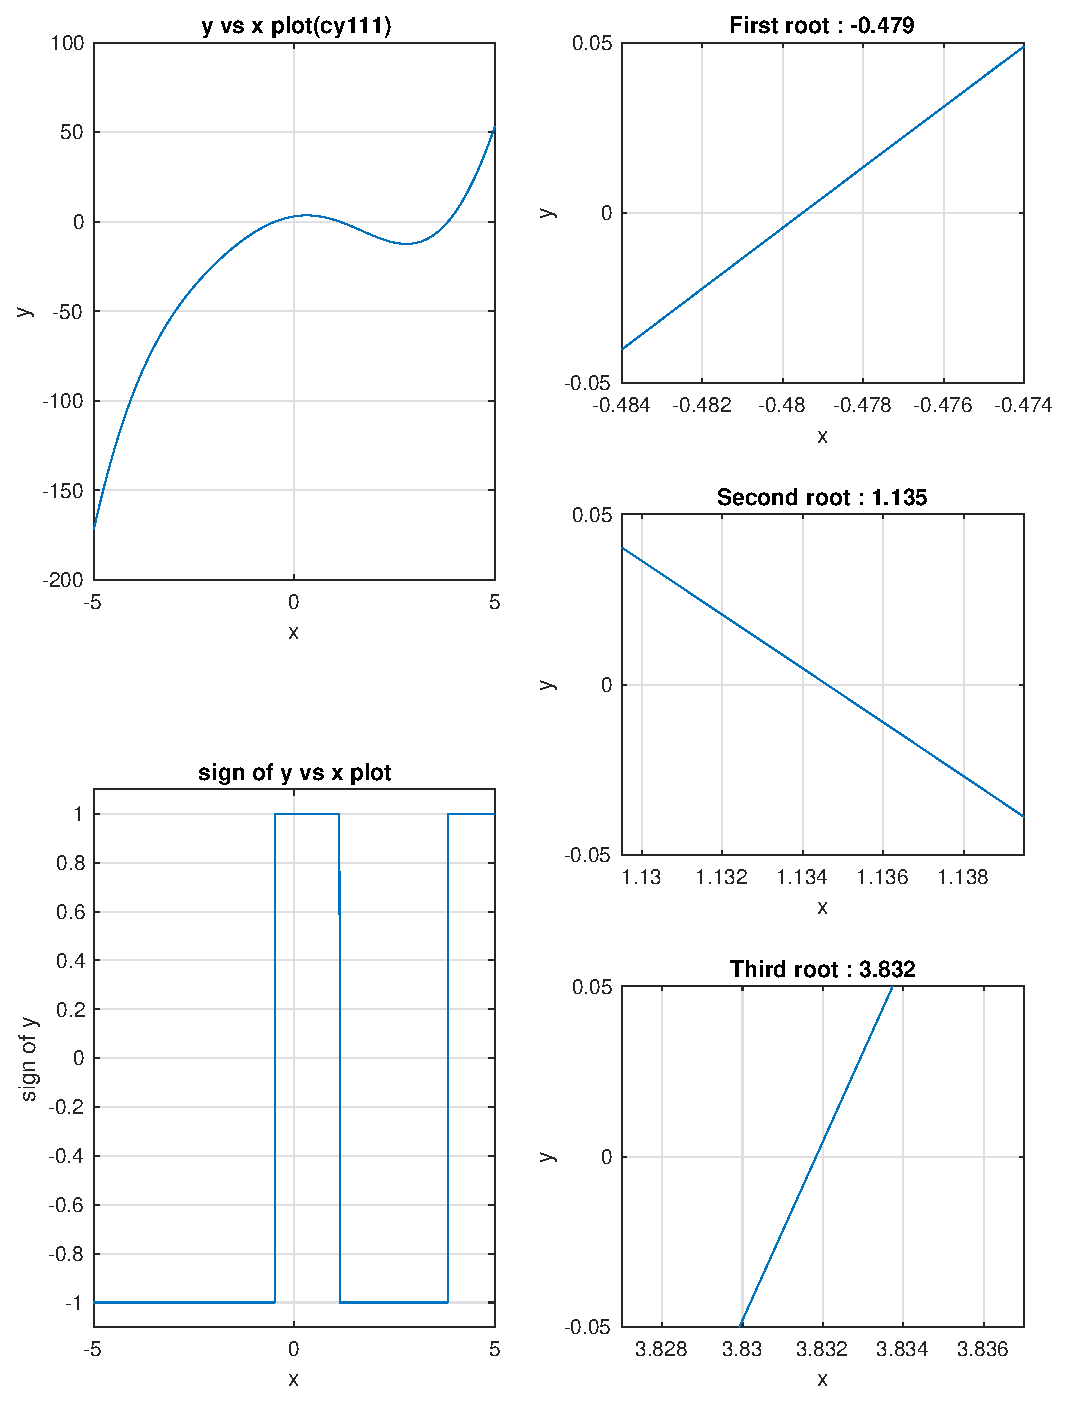
\epsfig{file=ThreeRoots.eps, width=3.5in} 
\caption{Palm Problem 5.3(a)}
\end{center}
\end{figure}

\begin{figure}[htb!]
\begin{center}
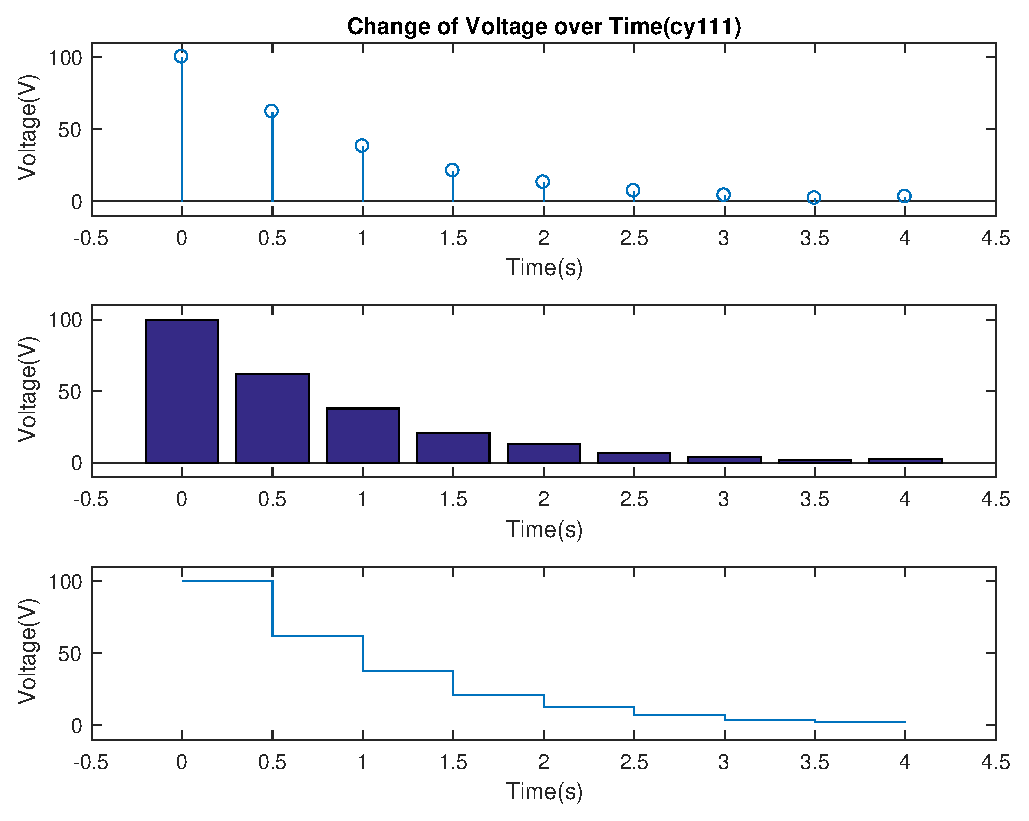
\epsfig{file=VoltageCalc.eps, width=3.5in} 
\caption{Palm Problems 5.21 and 6.7}
\end{center}
\end{figure}

\begin{figure}[htb!]
\begin{center}
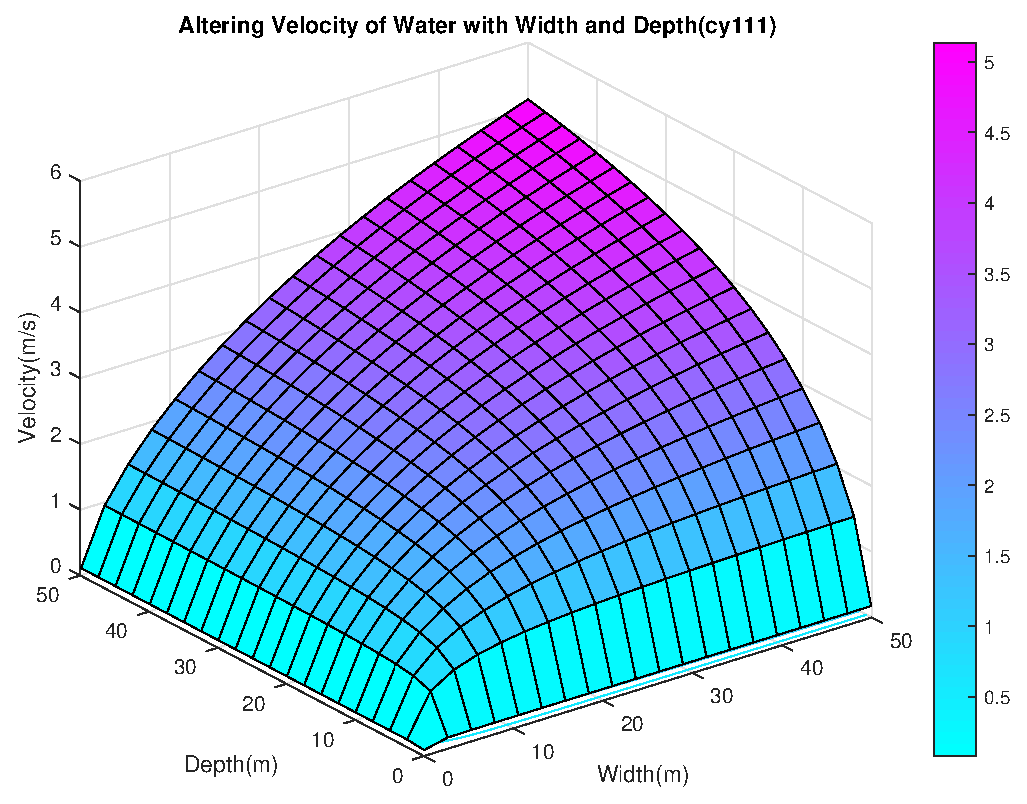
\epsfig{file=WaterVelocity.eps, width=3.5in} 
\caption{Chapra Problem 3.9}
\end{center}
\end{figure}


\begin{figure}[htb!]
\begin{center}
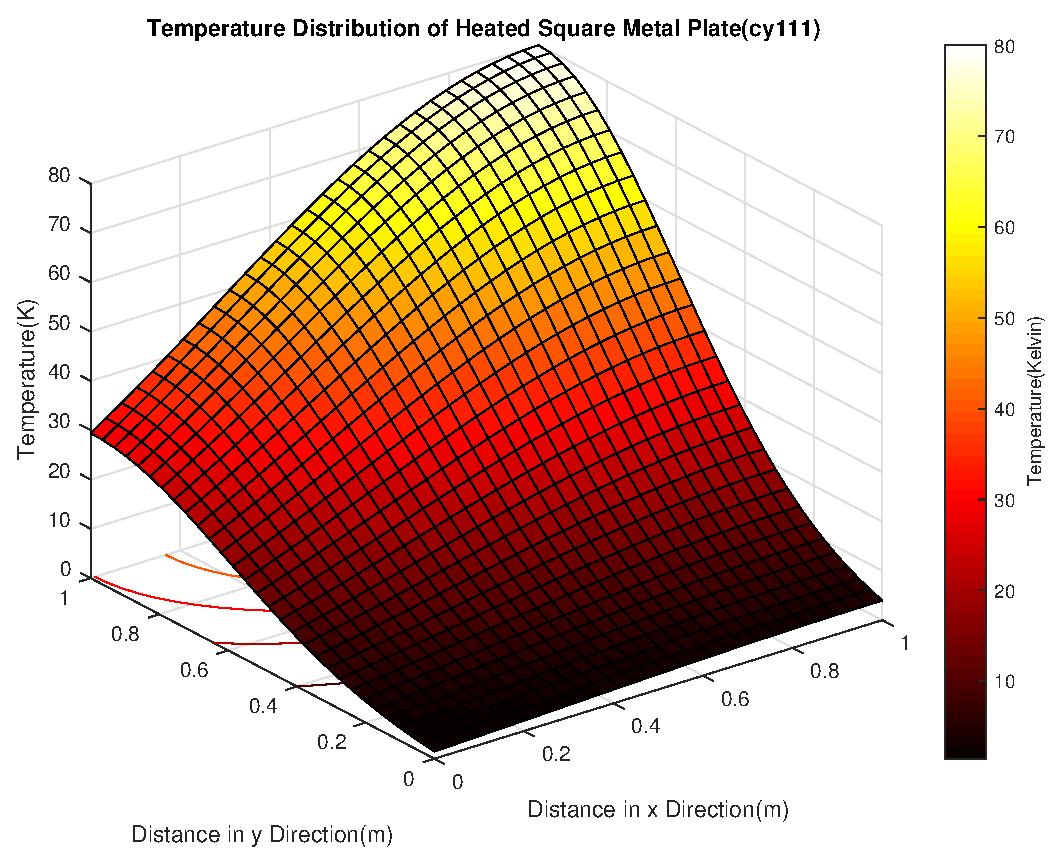
\epsfig{file=TemperatureDistribution.eps, width=3.5in} 
\caption{Palm Problem 5.33}
\end{center}
\end{figure}

\begin{figure}[htb!]
\begin{center}
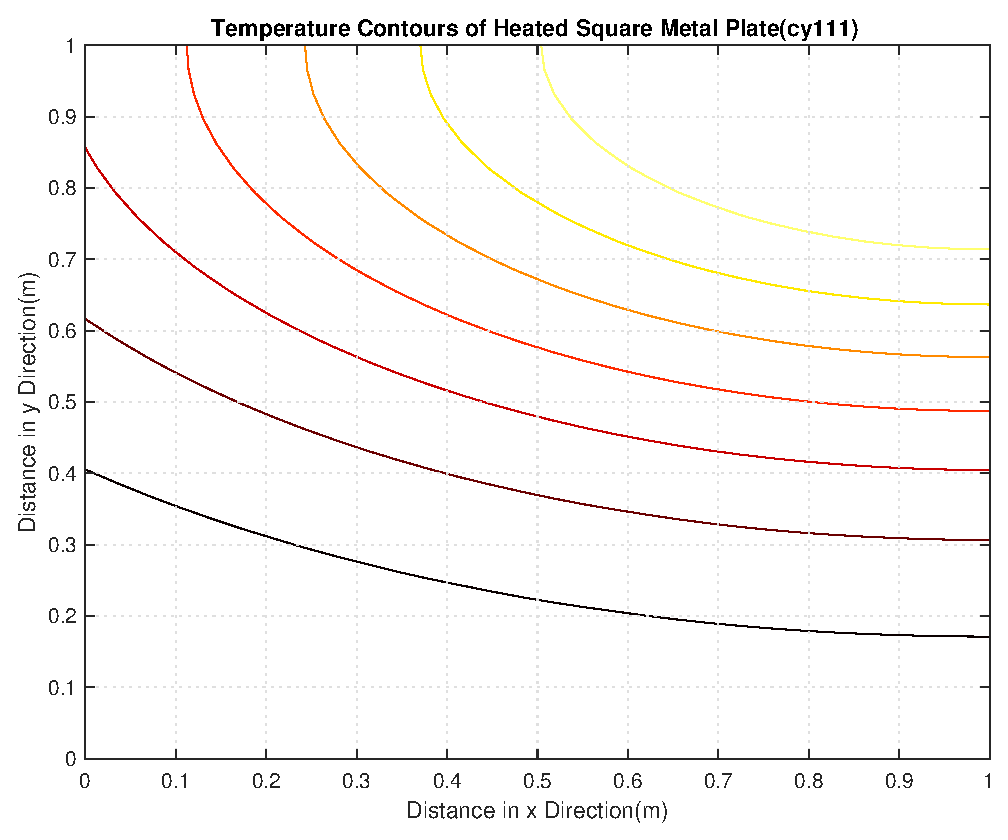
\epsfig{file=TemperatureContours.eps, width=3.5in} 
\caption{Palm Problem 5.33}
\end{center}
\end{figure}

\begin{figure}[htb!]
\begin{center}
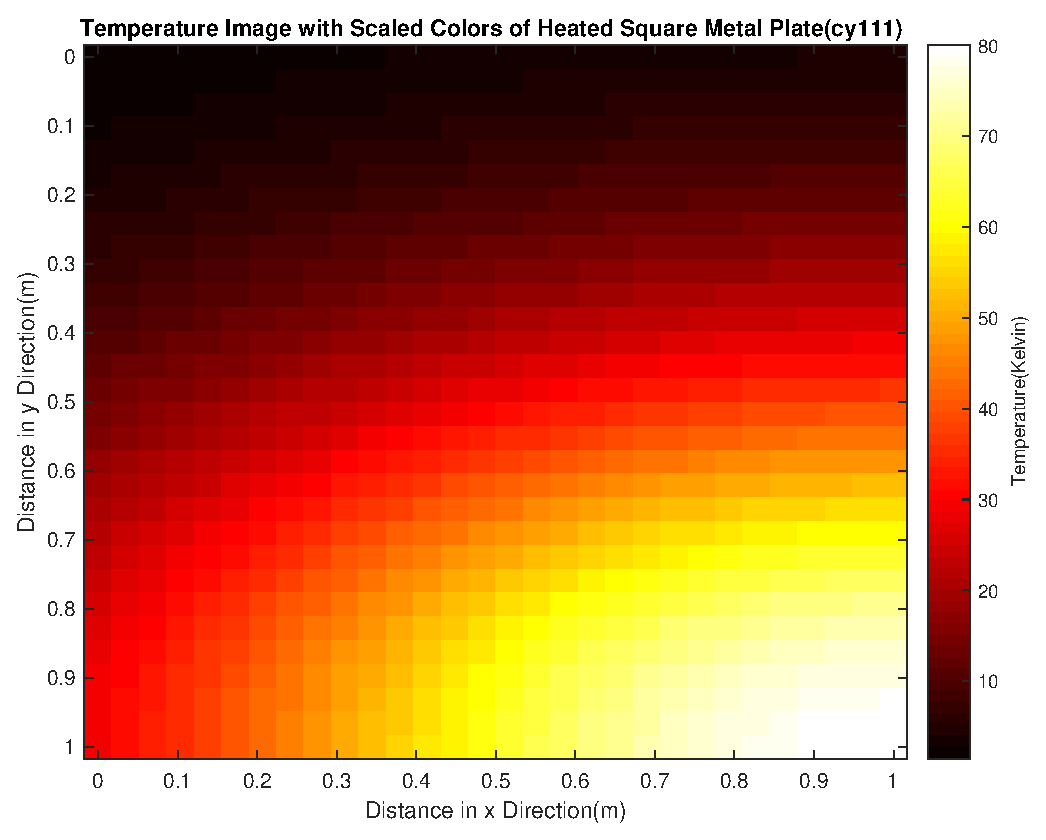
\epsfig{file=TemperatureImage.eps, width=3.5in} 
\caption{Palm Problem 5.33}
\end{center}
\end{figure}

\begin{figure}[htb!]
\begin{center}
\epsfig{file=ElectricPotentialSurface.eps, width=3.5in} 
\caption{Palm Problem 5.36}
\end{center}
\end{figure}

\begin{figure}[htb!]
\begin{center}
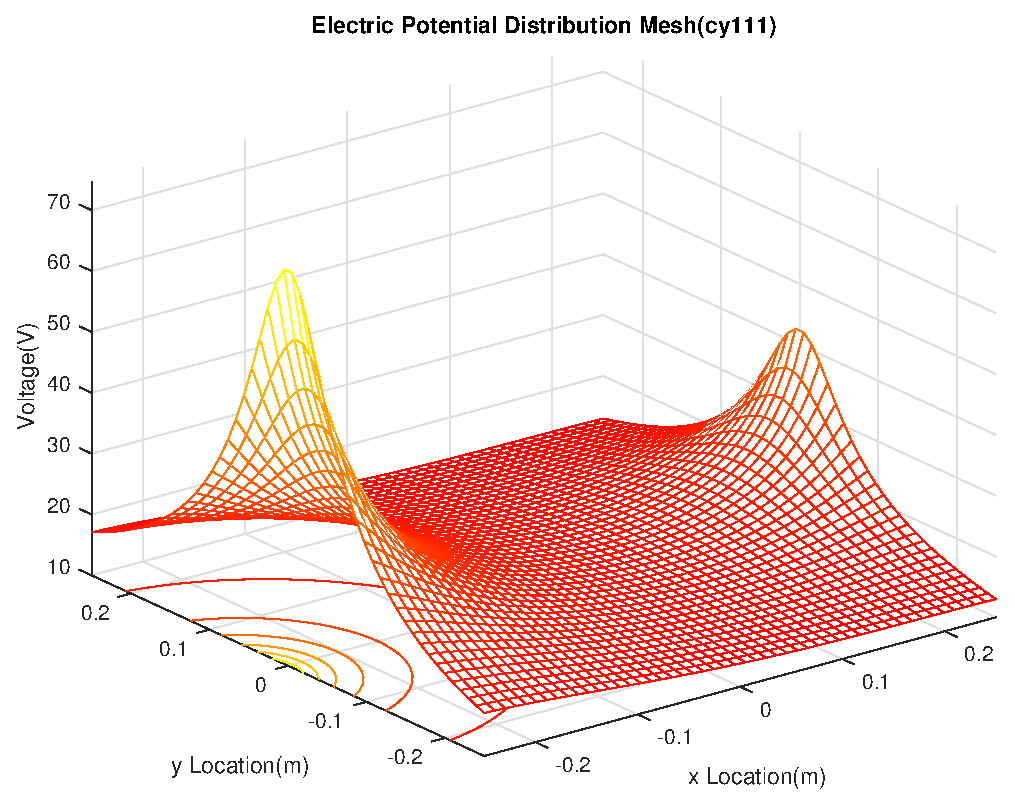
\epsfig{file=ElectricPotentialMesh.eps, width=3.5in} 
\caption{Palm Problem 5.36}
\end{center}
\end{figure}

\begin{figure}[htb!]
\begin{center}
\epsfig{file=DisCustomerLocations.eps, width=3.5in} 
\caption{Palm Problem 4.28}
\end{center}
\end{figure}

\begin{figure}[htb!]
\begin{center}
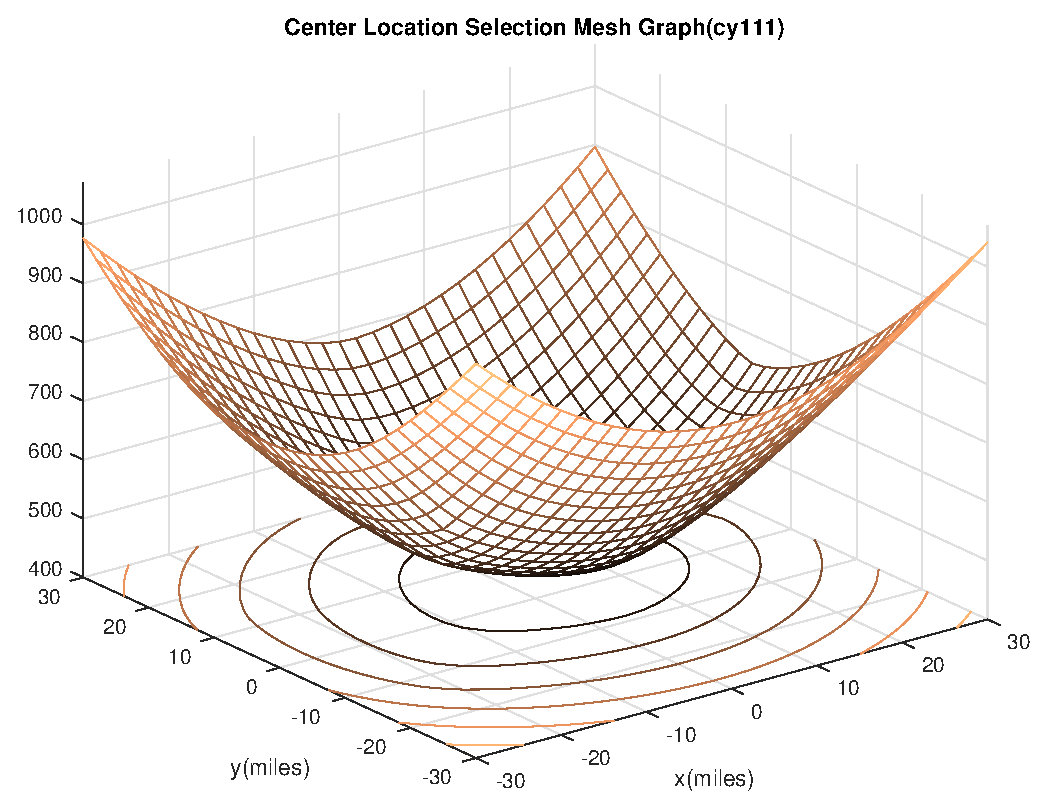
\epsfig{file=DisCenterMesh.eps, width=3.5in} 
\caption{Palm Problem 4.28}
\end{center}
\end{figure}

\begin{figure}[htb!]
\begin{center}
\epsfig{file=DisCenterSurface.eps, width=3.5in} 
\caption{Palm Problem 4.28}
\end{center}
\end{figure}

\begin{figure}[htb!]
\begin{center}
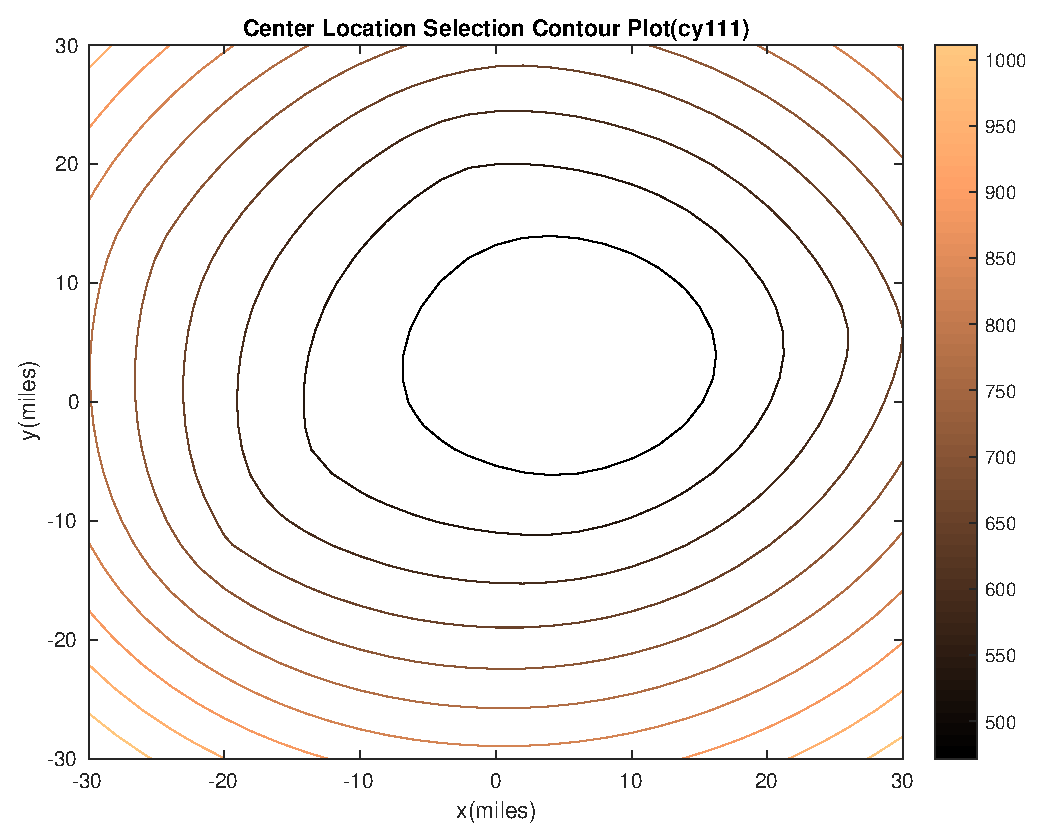
\epsfig{file=DisCenterContour.eps, width=3.5in} 
\caption{Palm Problem 4.28}
\end{center}
\end{figure}

\pagebreak

\begin{thebibliography}{9}
% You're welcome
\bibitem{Chapra}
  Chapra, Steven C.,
  {\it Applied Numerical Methods with MATLAB for Engineering and Scientists}.
  McGraw-Hill, New York,
  3rd Edition,
  2012.
\bibitem{Palm}
  Palm, William J.,
  {\it Introduction to MATLAB for Engineers}.
  McGraw-Hill, New York,
  3rd Edition,
  2011.
\end{thebibliography}

\end{document}

